\paragraph[QuizziPedia::Front-End::ModelViews\\::ConnectionQuestionsModelView]{QuizziPedia::Front-End::ModelViews::ConnectionQuestionsModelView}
\begin{figure} [ht]
	\centering
	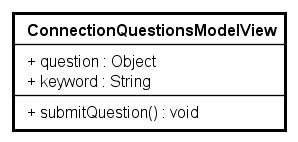
\includegraphics[scale=0.80]{UML/Classi/Front-End/QuizziPedia_Front-end_ModelView_ConnectionQuestionsModelView.png}
	\caption{QuizziPedia::Front-End::ModelViews::ConnectionQuestionsModelView}
\end{figure} \FloatBarrier
\begin{itemize}
	\item \textbf{Descrizione}: classe di tipo modelview la cui istanziazione è contenuta all'interno della variabile di ambiente \texttt{\$scope} di \textit{Angular\ped{G}}. All'interno di essa sono presenti le variabili e i metodi necessari per il \textit{Two-Way Data-Binding\ped{G}} tra la \textit{view\ped{G}} \texttt{ConnectionQuestionsView} e il \textit{controller\ped{G}} \texttt{ConnectionQuestionsController}; 
	\item \textbf{Utilizzo}: viene utilizzata per effettuare il \textit{Two-Way Data-Binding\ped{G}} tra la \textit{view\ped{G}}\\ \texttt{ConnectionQuestionsView} e il \textit{controller\ped{G}} \texttt{ConnectionQuestionsController} rendendo disponibili variabili e metodi;
	\item \textbf{Relazioni con altre classi}:
	\begin{itemize}
		\item \textbf{IN \texttt{ConnectionQuestionsView}}: \textit{view\ped{G}} contenente i campi e le direttive per creare una domanda a collegamento; 
		\item \textbf{IN \texttt{ConnectionQuestionsController}}: questa classe permette di gestire la creazione e la modifica di una domanda a collegamento.
	\end{itemize}
	\item \textbf{Attributi}:
	\begin{itemize}
		\item \texttt{+ question: Object} \\ Oggetto contenente gli attributi per la creazione della domanda:
		\begin{itemize}
			\item \texttt{answer: Array} \\ \texttt{array} contenente oggetti che rappresentano le risposte. Ogni oggetto risposta contiene:
			\begin{enumerate}
				\item \texttt{text1}: di tipo \texttt{String}, rappresenta il primo elemento testuale che sarà collegato ad un secondo elemento (testuale o immagine);
				\item \texttt{text2}:  di tipo \texttt{String}, rappresenta il secondo elemento testuale che sarà collegato al primo elemento (testuale o immagine);
				\item \texttt{url1}: di tipo \texttt{String}, rappresenta il primo elemento immagine che sarà collegato con il secondo elemento (testuale o immagine);
				\item \texttt{url2}: di tipo \texttt{String}, rappresenta il secondo elemento immagine che sarà collegato con il primo elemento (testuale o immagine).
			\end{enumerate}
		\end{itemize}
		\item \texttt{+ keyword: String} \\ Attributo contenente la keyword associata alla domanda/questionario;		
	\end{itemize}
	\item \textbf{Metodi}:
	\begin{itemize}
		\item \texttt{+ submitQuestion(): void}\\ 
		Metodo che gestisce l’evento click sul pulsante di conferma sulla domanda. Raccoglie i dati dal modelview e li manda al server attraverso \texttt{QuestionService}. Poi verrà effettuato il redirect alla pagina di gestione delle domande oppure al questionario che si stava creando.  
	\end{itemize}
\end{itemize}

